\section*{Introduction}

Developed economies require the continuous flow of persons and goods in astounding volumes. Transportation systems serve to enable these flows by minimizing friction. An effective transportation system is one which allows the economy to function with minimal losses. Encompassing this paradigm is the field of transportation accessibility. Transportation accessibility is the study of two related phenomena. (1) how structural and individual factors create latent flows or demand. (2) how efficiently transportation systems accommodate said flows. Economic growth, diversification, and specialization increase transportation demand. More efficient built environments and transportation systems reduce the cost of meeting demand. The interaction between economic development and transportation system development is reinforcing up to a saturation point. With the development and proliferation of new transportation technologies, the ultimate impacts on accessibility are important to measure.

Transportation accessibility measurement is a network problem. Any method which seeks to quantify accessibility must define the nodes and edges which comprise the region in question. In the modern world, all nodes are, to a greater or lesser extent, connected. It is often the case that several modes and paths can be nearly equal in cost. Scoping an accessibility analysis can be highly determinative of outcome. Researchers and planners have primarily utilized the concept of transportation accessibility as it applies to routine household behavior and local travel \cite{Handy_2020}. From the personal transportation perspective, access is defined as the ease with which individuals can reach the opportunities they desire subject to land-use, transportation infrastructure, temporal availability, and individual preference. Land-use dynamics determine the spatial distribution of amenities such as jobs and services as well as that of potential customers. Transportation systems determine the edge traversal costs including travel time, effort, and price which impede flows \cite{Geurs_2004}. Temporal availability of opportunities and transportation modes restrict the utility of opportunities and transportation modes. Characteristics such as age, income, and education predict attraction of opportunities and transportation modes of individuals \cite{Miller_2018}. Any transportation accessibility analysis must, thus, be stochastic.

Regions will vary both in infrastructure and resident preferences. The US and similar western nations are unusually car-centric by global standards  \cite{PrietoCuriel_2024}. Car dependence will not vanish in a short period. The differences between different types of car are important to consider. The access provided by a road transportation system for \gls{bev} drivers is different than that for \gls{icev} drivers due to vehicular and supply network characteristics. Modern \glspl{bev} possess sufficient practical ranges to accomplish much daily of daily travel as shown in Figure \ref{fig:utility_factors} with data from \cite{NHTS_2017, NHTS_2022}. However, for long itineraries \glspl{icev} offer greater accessibility compared to \glspl{bev} due to greater maximum ranges and the ubiquitous availability of fueling stations. Fueling stations are widely distributed across urban, suburban, and rural areas, ensuring that drivers have convenient access to refueling points wherever they travel. In contrast, the  charging network is less developed and distributed. This infrastructure gap poses challenges for \gls{bev} drivers, especially in remote or less densely populated areas, leading to range anxiety and limitations on travel options. Inadequate long-trip accessibility for \gls{bev} may result in cancellations or mode switches, often favoring \gls{icev} or air travel. By the same token, the lower operating costs of \glspl{bev} may cause short trips to be increasingly shifted towards them.

\begin{figure}[H]
	\centering
	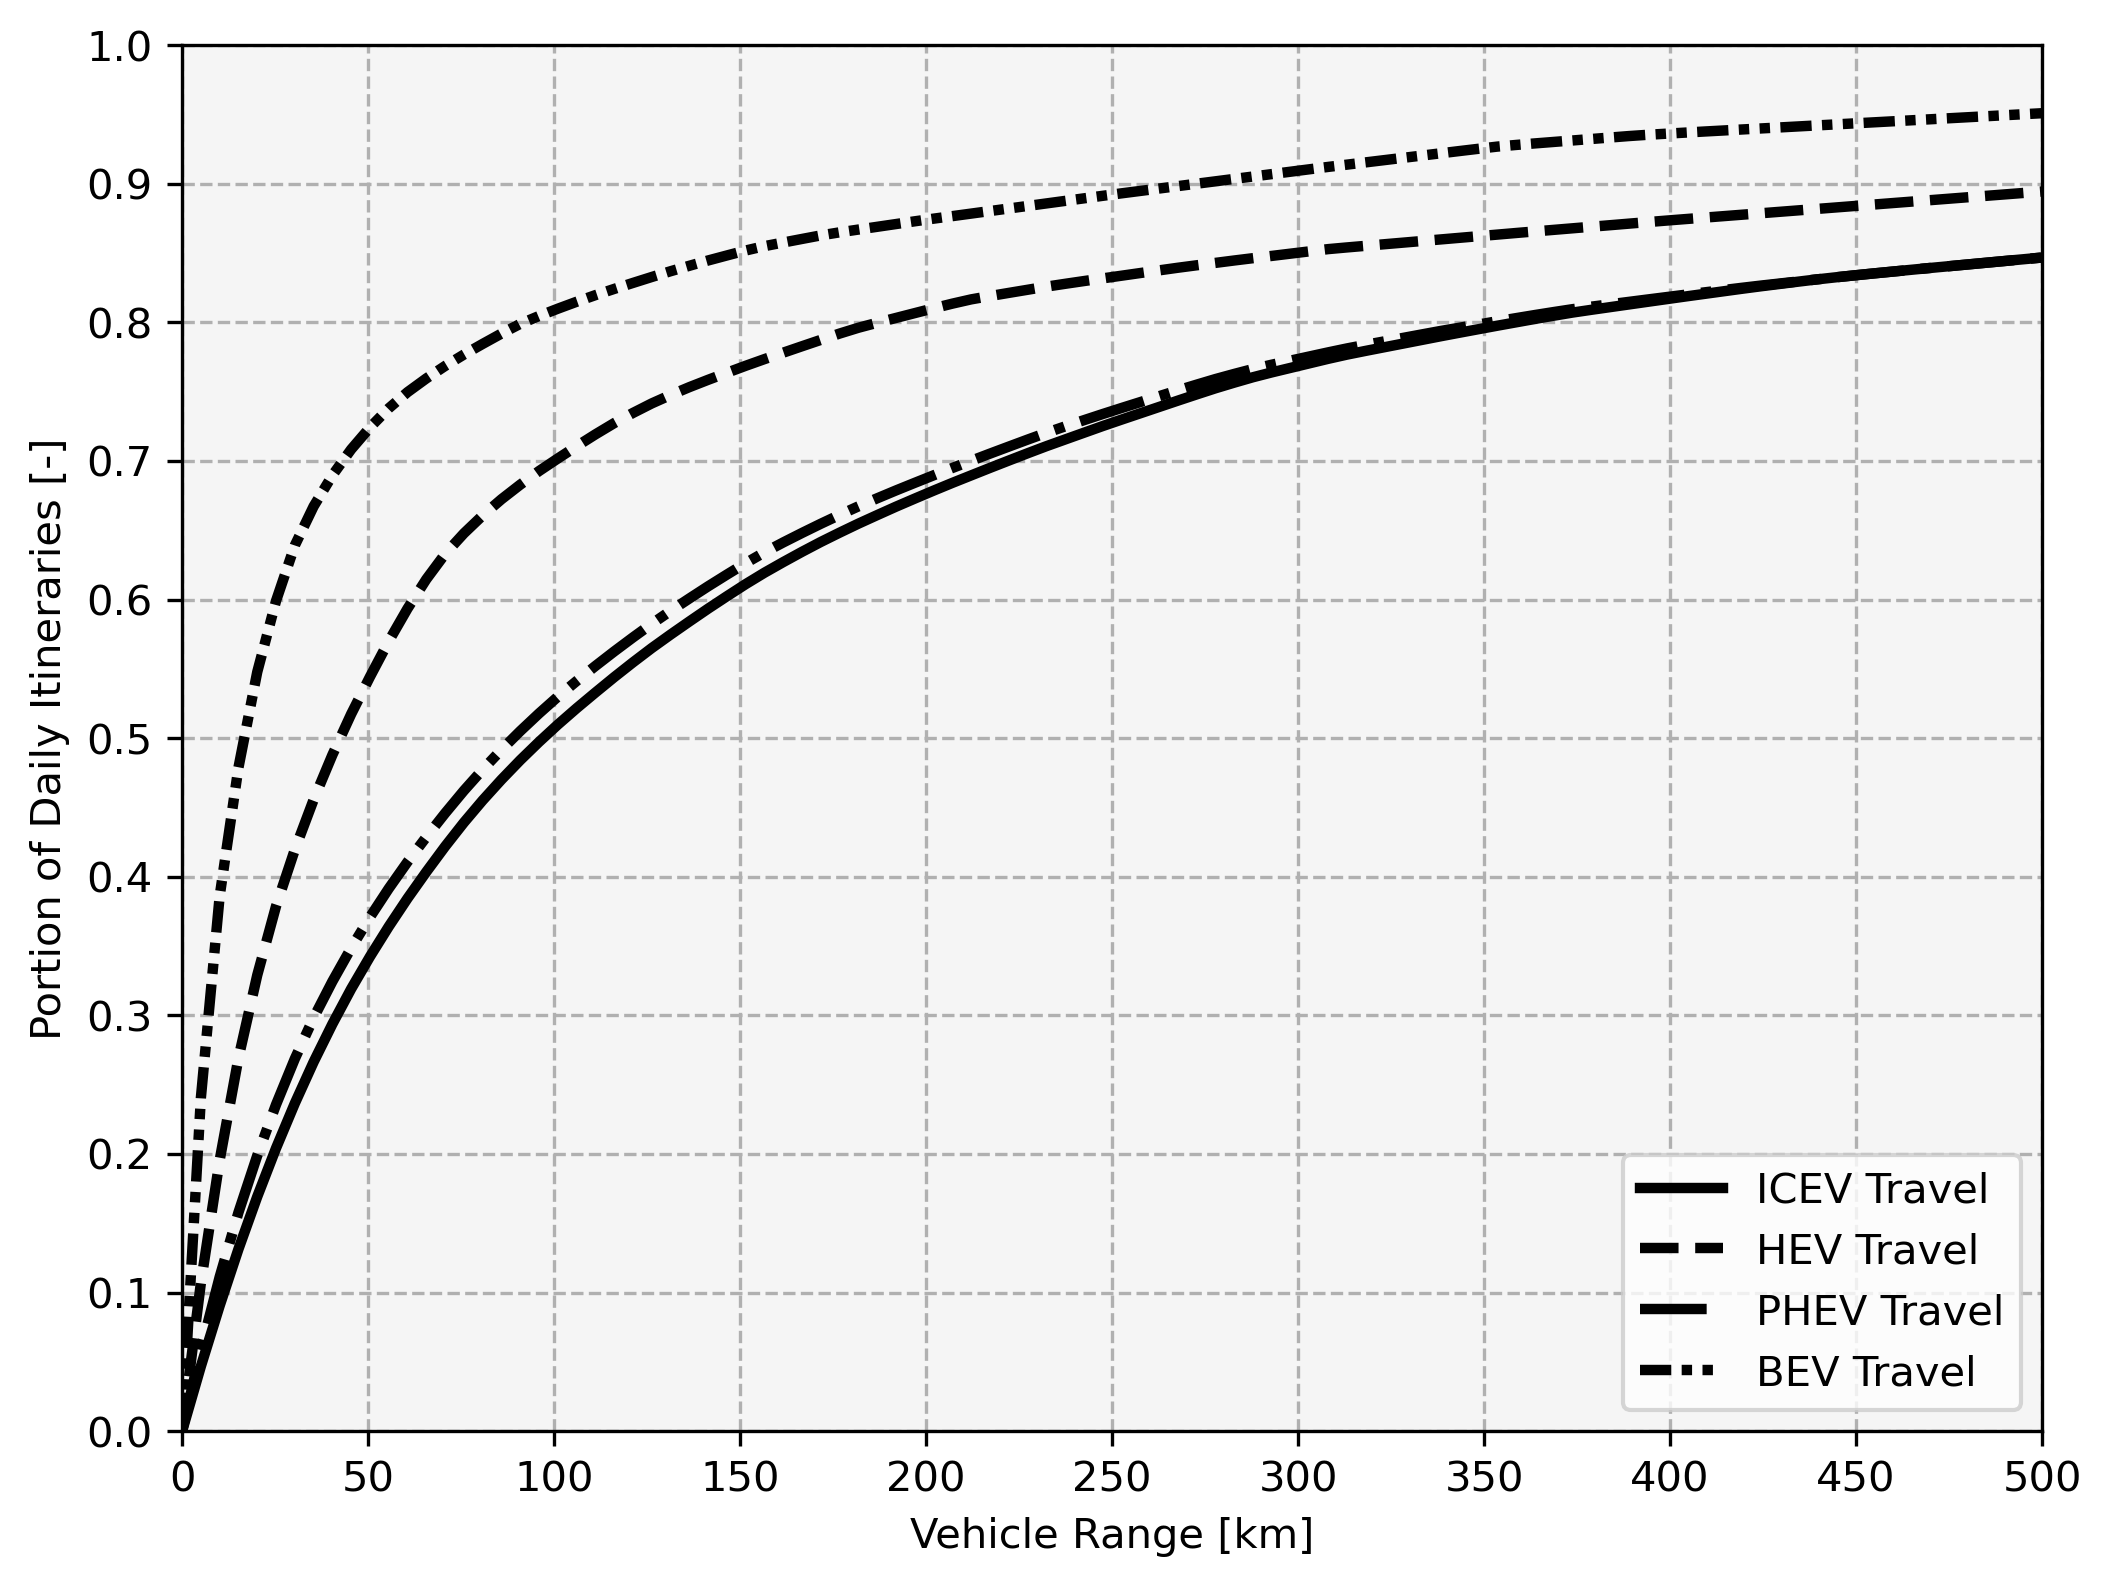
\includegraphics[width = \linewidth]{figs/UF_2022_km.png}
	\caption{Individual vehicle routine travel utility factors as a function of range by powertrain type for \gls{nhts} 2022 edition}
	\label{fig:utility_factors}
\end{figure}

Disparities between the fueling and DC charging networks result from differences in their underlying economic models. Gas pumping equipment requires lower up-front costs than DC \gls{evse}, is cheaper to operate \cite{Gamage_2023}, and has been deployed for far longer. Gas is often sold at low margin with stations making most profit on convenience items. Nearly all light-duty \gls{icev} drivers source all of their fuel from public fueling stations regardless of travel behavior. \gls{bev} drivers are expected to, and currently do, source much of their electricity from AC supply equipment during long dwells \cite{Hardman_2018}. These long dwells often take place at private chargers. Thus DC charging stations are subject to higher capital expenditure, lower revenue potential, and less accumulated investment. To overcome these disadvantages, public investments in DC charging infrastructure must be made judiciously. Evaluation methods for potential charging stations should consider their network-wide impact on accessibility considering vehicle types, equipment reliability, and driver behavior.

This study introduces a novel framework for the assessment of transportation accessibility for long vehicular trips. The methodology measures accessibility by computing optimal-feasible travel routes for \gls{od} pairs using a stochastic routing algorithm subject to vehicle range limitations, supply infrastructure, and driver risk attitudes. This methodology is powertrain agnostic and can be used to directly compare accessibility for vehicles with different ranges and which rely on different supply networks. Additionally, a case study is presented for the state of California showing a comparison between \glspl{icev} and \glspl{bev} access for important \gls{od} pairs within the state. The methodology introduced, as well as the open-source code provided in the supplemental information is a valuable tool for planners and policymakers in originating and evaluating \gls{evse} deployment policies.